\section{The empirical model quotient}
\label{sec:empiricalquotient}

Empirical equivalence partitions generative models into classes with equal reachable observation sets. The empirical model quotient records only this accessible information. The descent results use the same representative-independence principle as ordinary quotient constructions and universal properties \parencite{MacLaneBirkhoff1999,Leinster2014}, now applied to a space of models.

\begin{definition}[Empirical model quotient]
Let \(\mathfrak M_O\) denote the collection of generative models over \(O\), with a fixed set theoretic universe for latent spaces. The Lean development makes the corresponding universe parameters explicit. The empirical model quotient is
\[
\mathfrak M_O/{\approx},
\]
where \(\Model\approx\Model'\) means \(\Obs(\Model)=\Obs(\Model')\).
\end{definition}
The canonical projection sends each model to its empirical class:
\[
q_{\Emp}:\mathfrak M_O\to\mathfrak M_O/{\approx}.
\]
Two canonical classes are equal exactly when the corresponding models are empirically equivalent.

\subsection{Invariant properties descend}

\begin{theorem}[Universal property for model properties]
A property \(P:\mathfrak M_O\to\{\mathrm{false},\mathrm{true}\}\) is observation invariant if and only if there exists a unique property
\[
\bar P:\mathfrak M_O/{\approx}\to\{\mathrm{false},\mathrm{true}\}
\]
such that
\[
P=\bar P\circ q_{\Emp}.
\]
\end{theorem}

\begin{proof}
If \(P\) is observation invariant, define \(\bar P([\Model])=P(\Model)\). This is well defined because all representatives of one class have the same truth value. The factorization follows from the definition, and uniqueness follows because every quotient class has a representative. Conversely, any property factored through the quotient is constant on each quotient class and is therefore observation invariant.
\end{proof}
The same result holds for arbitrary valued measurements.

\begin{theorem}[Universal property for invariant measurements]
Let \(F:\mathfrak M_O\to V\). The map \(F\) assigns equal values to empirically equivalent models if and only if there exists a unique
\[
\bar F:\mathfrak M_O/{\approx}\to V
\]
such that \(F=\bar F\circ q_{\Emp}\).
\end{theorem}
\begin{figure}[tbp]
\centering
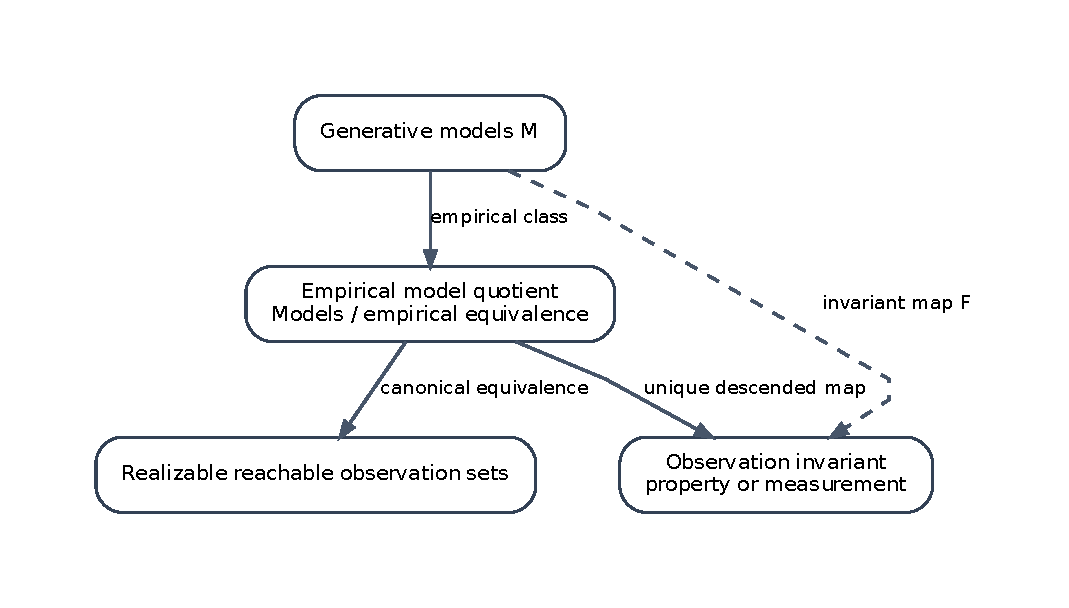
\includegraphics[width=0.86\textwidth]{figures/concept_empirical_quotient.pdf}
\caption{Empirical quotient and invariant descent. Observation invariant properties and measurements factor uniquely through empirical classes. Exact latent reconstructability fails this condition because it varies among representatives of one class.}
\label{fig:empiricalquotient}
\end{figure}

\subsection{Realizable observation sets}

The quotient has a concrete representation.

\begin{definition}[Realizable observation set]
A subset \(A\subseteq O\) is realizable when there exists a generative model \(\Model\) such that
\[
\Obs(\Model)=A.
\]
\end{definition}
\begin{theorem}[Canonical representation of empirical classes]
The map
\[
[\Model]\longmapsto\Obs(\Model)
\]
is a bijection between the empirical model quotient and the collection of realizable reachable observation sets.
\end{theorem}

\begin{proof}
The map is well defined because empirically equivalent models have equal reachable sets. It is injective because equal reachable sets imply empirical equivalence and therefore equal quotient classes. It is surjective by the definition of realizability.
\end{proof}
Each empirical class therefore specifies one reachable set. Whether a latent property is fixed within that class depends on the allowed models. For example, an empty reachable set forces an empty latent space.

\subsection{Exact reconstruction does not descend}

\begin{theorem}[Exact latent reconstruction is not a quotient property]
Assume \(O\neq\varnothing\) and a model class containing \((O,\id_O)\) and its Boolean hidden extension. Exact latent reconstructability does not factor through the empirical model quotient of that class.
\label{thm:decoderdoesnotdescend}
\end{theorem}

\begin{proof}
Use the identity model on \(O\); it is inhabited and has the identity decoder. Its Boolean hidden extension is empirically equivalent to the base. The extension has a noninjective observation map and no exact latent decoder. Therefore the property has different truth values on two representatives of one empirical class. A property with that variation cannot descend to the quotient.
\end{proof}
The identity model gives a counterexample at the full observation space. An inclusion map gives a counterexample at any prescribed nonempty reachable set.

\begin{corollary}[Decoder status at a prescribed reachable set]
Let \(\varnothing\ne S\subseteq O\). If the model class contains the inclusion \(i:S\hookrightarrow O\) and its Boolean extension, the empirical class for \(S\) contains both an exactly decodable model and one without a decoder. If the reachable set is empty, all compatible models have the same decoder status.
\end{corollary}

\begin{proof}
Choose \(s_0\in S\). The map \(d:O\to S\) that returns \(o\) for \(o\in S\) and \(s_0\) otherwise satisfies \(d\circ i=\id_S\). Its Boolean extension reaches the same set, and \((s_0,0)\) and \((s_0,1)\) prevent exact decoding. If the reachable set is empty, a source state would give a reachable value, so the source is empty. A total map from \(O\) into the empty set exists precisely when \(O\) is empty.
\end{proof}
